\documentclass[10pt,twocolumn,twoside,letterpaper]{IEEEtran}

\usepackage[spanish]{babel}
\usepackage{amsmath}
\usepackage{graphics}
\usepackage{graphicx}
\usepackage{color}
\usepackage{anysize}

%\setlength{\oddsidemargin}{1cm}
%\setlength{\evensidemargin}{0.25mm}
%\setlength{\topmargin}{0.37cm}
\setlength{\textwidth}{15.6cm}
\setlength{\columnsep}{1.19cm}
\setlength{\textheight}{23cm}
%\pagestyle{headings} %%Encabezados

\marginsize {3.5cm}{2.5cm}{3.2cm}{-.05cm}
\bibliographystyle{/home/rsheissa/papers/inaoe_investigation/ieeebib}

%opening
\title{Jerarqu\'ia en Expresiones de Ruido para Amplificadores con Uno y Dos Lazos de Retroalimentaci\'on Basados en Nullor}
\author{\begin{Large}{Roberto Casta\~neda Sheissa}\end{Large}\\ \begin{Large}Instituto Nacional de Astrof\'isica, \'Optica y Electr\'onica\end{Large}\\ \begin {Large} Departamento de Electr\'onica, Grupo de CAD\end{Large}\\ \begin{Large}P.O. Box 51, 72000, Puebla, Pue., M\'exico\end{Large}\\ \begin{Large}Email: {\tt rsheissa@inaoep.mx}\end{Large}}

\begin{document}

\pagestyle{empty}
\maketitle

\thispagestyle{empty}
\begin{abstract}
El presente trabajo muestra la jerarqu\'ia existente en las expresiones de ruido equivalente a la entrada para amplificadores cuyo dise\~no se basa en nullor. Las expresiones presentadas son para amplificadores de un lazo y dos lazos de retroalimentaci\'on. Tales expresiones pueden ser codificadas me\-dian\-te un lenguaje de programaci\'on a fin de incluirlas en una herramienta de dise\~no automatizado.
\end{abstract}

{\section{\bf {INTRODUCCI\'ON}}
La teor\'ia de dise\~no estructurado \cite{verhoeven,verhoeven1} permite realizar dise\~no partiendo del principio que existe una {\it soluci\'on ideal}. A partir de esta soluci\'on ideal se realiza la s\'intesis necesaria para llegar a un resultado particular, en otras palabras, el resultado final es un circuito con elementos reales. Gr\'aficamente se puede visualizar el concepto en la figura \ref{fig:dis_est}.

\begin{figure}[hbtp]
   \centering
   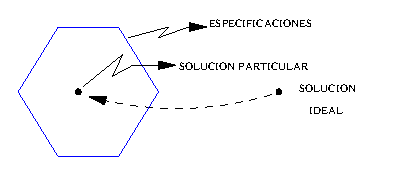
\includegraphics[scale=.9]{/home/rsheissa/papers/inaoe_investigation_2004/figuras/dis_est.eps}
   \caption{Dise\~no Estructurado}
   \label{fig:dis_est}
\end{figure}

\section{\textbf{EL NULLOR}}
Para el dise\~no de amplificadores, el dise\~no estructurado utiliza el concepto de nullor como el elemento para alcanzar la soluci\'on ideal. Este elemento es un componente singular de dos puertos. En el puerto de entrada se encuentra un nullator y en el puerto de salida un norator, como se muestra en la figura \ref{fig:nullor}.

\begin{figure}[hbtp]
   \centering
   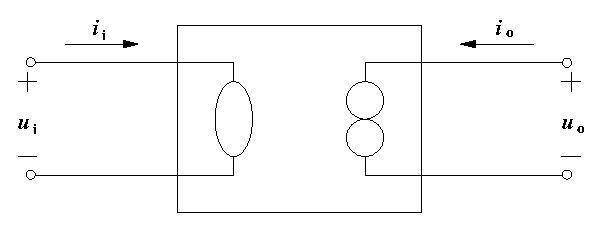
\includegraphics[scale=.6]{/home/rsheissa/papers/inaoe_investigation_2004/figuras/fig_nullor.eps}
   \caption{El Nullor}
   \label{fig:nullor}
\end{figure}

\vspace{-15mm}

A la entrada, el {\it nullator} tiene una relaci\'on de rama que vuelve cero la corriente y el voltaje, esto es $$i_i=0 \qquad u_i=0$$

Para el puerto de salida, el {\it norator} tiene una relaci\'on de rama que permite a ambas variables, voltaje y corriente, tomar cualquier valor, es decir $$i_o={\times} \qquad u_o={\times}$$ por lo tanto, las variables de salida del {\it nullor} est\'an definidas por el ambiente.

Una propiedad interesante del nullor que es sumamente \'util en el dise\~no de amplificadores es que su {\it matriz de la cadena} tiene la forma:

\begin{scriptsize}\begin{equation}
K=
\left[\begin{array}{cc}
A&B\\
C&D
\end{array} \right]=
\left[\begin{array}{cc}
0&0\\
0&0
\end{array} \right]
\end{equation}\end{scriptsize}

{\noindent esto significa que el {\it nullor} representa todos los tipos de funciones de transferencia teniendo ganancia muy alta, ninguna contribuci\'on de ruido y comportamiento que no depende de la frecuencia.}

Como resultado, el dise\~no estructurado de amplificadores consiste en una modificaci\'on sistem\'atica del nullor hasta realizar su completa s\'intesis con dispositivos reales, tales como son los transistores.

Es posible ver a un amplificador con retroalimentaci\'on negativa como la conexi\'on de dos bloques; el primer bloque se considera la planta a ser controlada y el segundo bloque es la {\it retroalimentaci\'on} del sistema. La planta es el {\it nullor} el cual ser\'a sintetizado utilizando dispositivos con ganancia alta, los \'unicos dispositivos que poseen esta caracter\'itica son los dispositivos activos. La red de retroalimentaci\'on est\'a formada por redes pasivas conteniendo resistores. 

\section{\textbf{DISE\~NO ESTRUCTURADO}}
Se han definido topolog\'ias b\'asicas de amplificadores con un lazo de retroalimentaci\'on mediante la combinaci\'on del {\it nullor} y componentes pasivos \cite{verhoeven,stoffels}, las cuales se presentan en la figura \ref{fig:basic_topologies}.

\begin{figure}[hbtp]
   \centering
   \includegraphics[scale=.45]{/home/rsheissa/papers/inaoe_investigation_2004/figuras/grupo.eps}
   \caption{Topolog\'ias B\'asicas de Un Lazo.}
   \label{fig:basic_topologies}
\end{figure}

La figura \ref{fig:basic_two_loops} muestra la topolog\'ia con dos lazos de retroalimentaci\'on \cite{stoffels}. Las matrices de transmisi\'on para las topolog\'ias b\'asicas de un lazo son las siguientes:

\begin{scriptsize}\begin{equation}
\begin{array}{ll}
{K_{V}=
\left[\begin{array}{cc}
{\frac{1}{1+R_1/R_2}}&0\\
0&0
\end{array} \right]}&
{K_{G}=
\left[\begin{array}{cc}
0&{-1/G}\\
0&0
\end{array} \right]}\\
\\
{K_{R}=
\left[\begin{array}{cc}
0&0\\
{-1/R}&0
\end{array} \right]}&
{K_{I}=
\left[\begin{array}{cc}
0&0\\
0&{\frac{1}{1+R_1/R_2}}
\end{array} \right]}
\end{array}
\label{eq:chain_matrix}
\end{equation}\end{scriptsize}

\begin{figure}
   \centering
   \includegraphics[scale=.4]{/home/rsheissa/papers/inaoe_investigation_2004/figuras/basic_two_loops.eps}
   \caption{Topolog\'ias B\'asicas de Dos Lazos con {\mbox Nullor}.}
   \label{fig:basic_two_loops}
\end{figure}

Las {\it matrices de transmisi\'on} para cada una de las topolog\'ias de dos lazos son las siguientes:

\begin{scriptsize}\begin{equation}
\begin{array}{l}
{K_{(A)}=
\left[\begin{array}{cc}
{\frac{R_1+R_2}{R_2}}&0\\
{\frac{(R_1+R_2)(R_3+R_4)}{R_2+R_3}}&{\frac{R_3+R_4}{R_4}}
\end{array} \right]}
\\
\\
{K_{(B)}=
\left[\begin{array}{cc}
{1-G_2R_1}&{\frac{1-G_2R_1}{R_1}}\\
{\frac{1-G_2R_1}{G_2}}&{1-G_2R_1}
\end{array} \right]}
\end{array}
\end{equation}
\end{scriptsize}
Las configuraciones de dos lazos son empleadas como acopladores de impedancias en entrada o salida \cite{nordholt}.

\begin{figure*}[!thbp]
\hrulefill
\begin{footnotesize}\begin{equation}
u_{n,v_{total}}=u_{ns}+u_{nn}+\biggl(R_s+\frac{R_1R_2}{R_1+R_2}\biggr)i_{nn}+\biggl(\frac{R_2}{R_1+R_2}\biggr)u_{nR_1}+\biggl(\frac{R_1}{R_1+R_2}\biggr)u_{nR_2}
\label{eq:noise_volt}
\end{equation}\end{footnotesize}

\begin{footnotesize}\begin{equation}
u_{n,v_{total}}=u_{ns}+u_{nn}+\Bigl(R_s+R\Bigr)i_{nn}+\Bigl(R\Bigr)i_{nR}
\label{eq:noise_transadm}
\end{equation}\end{footnotesize}

\begin{footnotesize}\begin{equation}
i_{n,i_{total}}=i_{ns}+i_{nn}+\biggl(\frac{1}{R_s}+\frac{1}{R_1+R_2}\biggr)u_{nn}+\\
\biggl(\frac{R_2}{R_1+R_2}\biggr)i_{nR_2}+\biggl(\frac{R_1}{R_1+R_2}\biggr)i_{nR_1}
\end{equation}\end{footnotesize}

\begin{footnotesize}\begin{equation}
i_{n,i_{total}}=i_{ns}+i_{nn}+\biggl(\frac{1}{R_s}+\frac{1}{R}\biggr)u_{nn}+\biggl(\frac{1}{R}\biggr)u_{nR}
\end{equation}\end{footnotesize}
\hrulefill
\end{figure*}

\begin{center}\subsection{{\bf RUIDO EN AMPLIFICADORES}}\end{center}
El ruido es un fen\'omeno que inevitablemente se encuentra en cualquier dise\~no electr\'onico no importando la con\-fi\-gu\-ra\-ci\'on ni los componentes. Aunque no es posible eliminarlo definitivamente es posible mantenerlo dentro de ciertos l\'imites, propuestos por el dise\~nador, siendo necesario conocer las contribuciones de todos los componentes del amplificador.

El mejor punto para medir el valor de ruido \mbox{total} es a la salida del amplificador, esto es lo que com\'unmente se realiza para obtener el valor modificado con respecto a la se\~nal de entrada. Desde el punto de vista del dise\~no de amplificadores el punto m\'as conveniente para realizar la medici\'on de la contribuci\'on de ruido es a la entrada del amplificador. Utilizando este concepto se puede obtener un valor de ruido representado por una fuente de voltaje, corriente o ambas. Esta o estas fuentes estar\'an fuera de la implementaci\'on del amplificador, es decir, se tiene un amplificador libre de ruido.

\begin{figure}[hbtp]
   \centering
   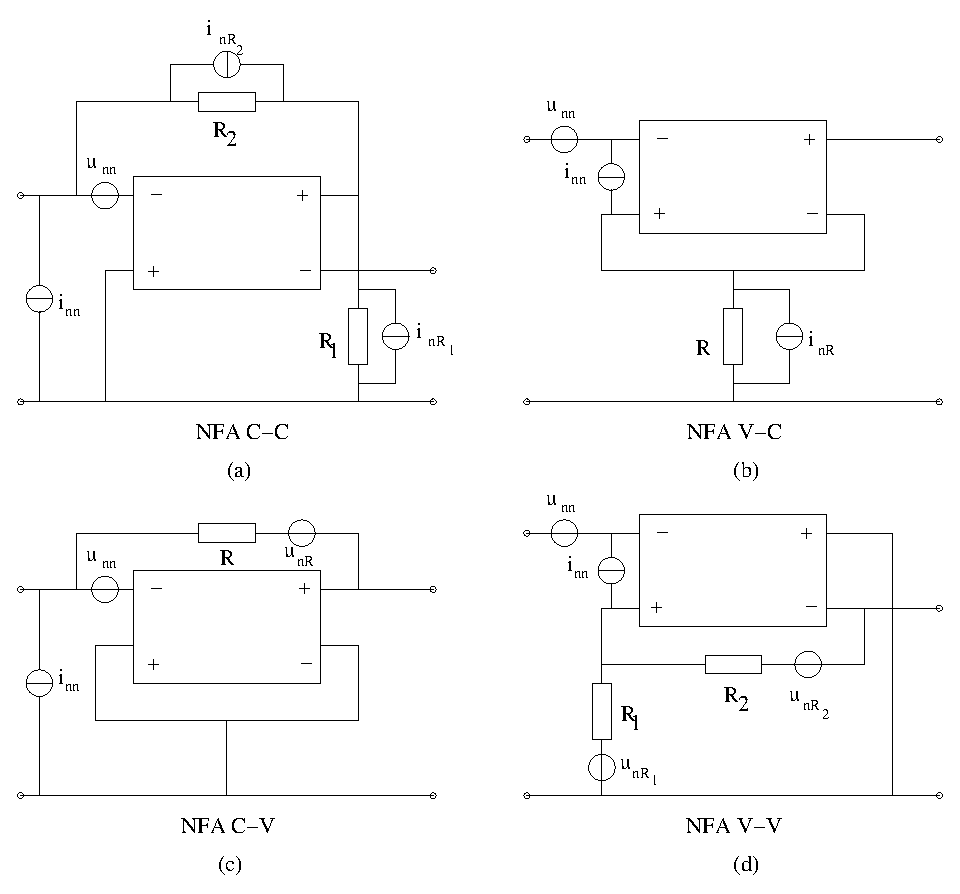
\includegraphics[scale=0.4]{/home/rsheissa/papers/inaoe_investigation_2004/figuras/grupo_noise.eps}
   \caption{Amplificador Un Lazo con Ruido}
   \label{fig:grupo_noise}
\end{figure}

Para obtener la contribuci\'on de ruido de todos los elementos utilizados en la s\'intesis e implementaci\'on del amplificador, es necesario mover las fuentes ruidosas hacia el exterior. Esto se realiza por medio de varias manipulaciones de fuentes \cite{verhoeven,nordholt}.
\\
\section{{\bf JERARQU\'IA DE EXPRESIONES}}
 Para las topolog\'ias de un solo lazo se obtiene una sola expresi\'on para cada una de ellas; para las topolog\'ias de doble lazo se obtienen dos expresiones debido a que estas configuraciones pueden ser excitadas tanto por fuentes de corriente o de voltaje y obtener corriente o voltaje a la salida.

\begin{figure}
   \centering
   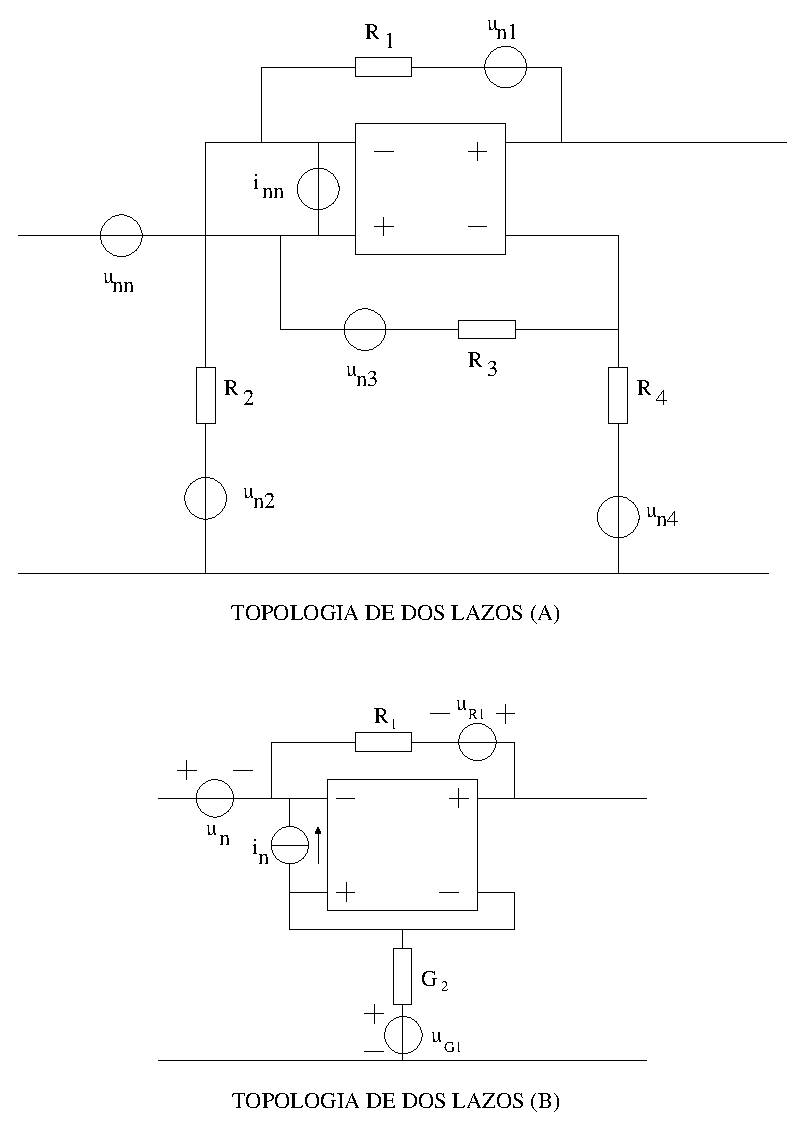
\includegraphics[scale=0.4]{/home/rsheissa/papers/inaoe_investigation_2004/figuras/twoloop_noise.eps}
   \caption{Amplificador Dos Lazos con Ruido}
   \label{fig:twoloop_noise}
\end{figure}

\subsection{{\bf Expresiones para Un Lazo}}
\label{sec:exp_1loop} Las expresiones a obtener de los ampificadores mostrados en la figura \ref{fig:grupo_noise} se clasifican dependiendo del tipo de fuente de excitaci\'on dando como resultado las siguientes ecuaciones de ruido: para el amplificador de voltaje (4), transconductancia (5), transimpedancia (6) y corriente (7).

\subsection{{\bf Expresiones para Dos Lazos}}
\label{sec:exp_2loop} Las topolog\'ias se muestran en la figura \ref{fig:twoloop_noise}, tomando en cuenta la nomenclatura mostrada en la figura se har\'a referencia a los amplificadores como (A) y (B) respectivamente. Las expresiones de ruido para (A) son (8) y (9), para (B) (10) y (11).

\begin{figure*}[!t]
\hrulefill
\begin{footnotesize}\begin{equation}
\label{Amplificador (A) excitado por Voltaje}
\begin{split}
u_{n,v_{total}(A)}=u_{ns}+u_{nn}+\biggl(R_S+R_2+\frac{R_SR_2}{R_3+R_4}\biggr)i_{nn}+\biggl(\frac{R_2}{R_1+R_2}+\frac{R_S(R_3+R_4)}{(R_1+R_2)(R_3+R_4)}\biggr)u_{nR_1}+\\
\biggl(1+\frac{R_S}{R_3+R_4}\biggr)u_{nR_2}+\biggl(\frac{R_S}{R_3+R_4}\biggr)u_{nR_3}+\biggl(\frac{R_S}{R_3+R_4}\biggr)u_{nR_4}
\end{split}
\end{equation}\end{footnotesize}
\begin{footnotesize}\begin{equation}
\begin{split}
i_{n,i_{total}(A)}=i_{ns}+i_{nn}+\biggl(G_S+\frac{1}{R_3+R_4}\biggr)u_{nn}+\biggl(\frac{R_1R_2G_S}{R_1+R_2}+\frac{R_1R_2+R_1R_4}{(R_1+R_2)(R_3+R_4)}\biggr)i_{nR_1}+\\
\biggl(R_2G_S+\frac{R_2}{R_3+R_4}\biggr)i_{nR_2}+\biggl(\frac{R_3}{R_3+R_4}\biggr)i_{nR_3}+\biggl(\frac{R_4}{R_3+R_4}\biggr)i_{nR_4}
\end{split}
\end{equation}\end{footnotesize}

\begin{footnotesize}\begin{equation}
\begin{split}
u_{n,v_{total}(B)}=u_{ns}+u_{nn}+\biggl(R_S+\frac{R_S+R}{1-GR}\biggr)i_{nn}+\biggl(\frac{1+GR_S}{1-GR}\biggr)u_{nR}+\biggl(\frac{G(R+R_S)}{1-GR}\biggr)u_{nG}
\end{split}
\end{equation}\end{footnotesize}
\vspace{-0.5mm}
\begin{footnotesize}\begin{equation}
\begin{split}
i_{n,i_{total}(B)}=i_{ns}+i_{nn}+\biggl(G_S+\frac{G_S+G}{1-GR}\biggr)u_{nn}+\biggl(\frac{R(G_S+G)}{1-GR}\biggr)i_{nR}+\biggl(\frac{1+G_SR}{1-GR}\biggr)i_{nG}
\end{split}
\end{equation}\end{footnotesize}
\hrulefill
\end{figure*}


\subsection{\textbf{Relaci\'on de Jerarqu\'ia}}
\label{sec:hierarchy}  Desde el punto de vista de dise\~no estructurado se ha partido desde el elemento ideal, se agreg\'o una red de retroalimentaci\'on y se anex\'o una exitaci\'on. Sobre el arreglo anterior se realizaron los c\'alculos para obtener el equivalente de ruido a la entrada tomando en cuenta todos los elementos que forman parte del circuito. En resumen se han recorrido los distintos niveles de jerarqu\'ia para el dise\~no de esta etapa del amplificador.

Al observar las expresiones obtenidas para uno y dos lazos de retroalimentaci\'on es posible notar las relaciones que entre ellas existen si se agrupan de tal forma que se puedan formar bloques. Agrupando los resultados en estos bloques es posible notar lo siguiente:

\begin{itemize}
\item {\bf Ruido de la Fuente.} Esta contribuci\'on es del mismo tipo de la variable de entrada del amplificador. Este dato es definido com\'unmente por la caracter\'istica de la resistencia de fuente, y por lo tanto es un valor que no puede ser modificado. Se denota como $u_{ns}$ \'o $i_{ns}$.
\item {\bf Ruido del nullor con la variable apropiada.} Este es el ruido de la s\'intesis del nullor expresado en el mismo valor que el ruido de la fuente. Puede ser $u_{nn}$ \'o $i_{nn}$. $u_{nn}$ est\'a conectada en serie e $i_{nn}$ en paralelo.
\item {\bf Ruido del nullor de la variable disjunta.} La contribuci\'on de ruido por la s\'intesis del nullor expresada como la ley de Ohm: $$u=(R_S+R_{eq})i_{nn}$$ \'o $$i=(G_S+G_{eq})u_{nn}$$ donde $R_S$ es la resistencia de fuente y $G_S=1/R_S$. Donde la contribuci\'on de $R_{eq}$ depende de los resistores con que se implementa la red de retroalimentaci\'on.
\item {\bf Ruido por la red pasiva.} Esta es la contribuci\'on de ruido por los resistores que conforman la red de retroalimentaci\'on. Para los amplificadores de voltaje y corriente de un solo lazo y el amplificador de dos lazos (B) involucran a dos resistores, para el amplificador de dos lazos (A) involucra a cuatro resistores; esto significan contribuciones significativas al ruido total del amplificador. Para el resto de los amplificadores, la ganancia est\'a determinada por un solo resistor, por lo tanto un \'unico termino aparece en la suma. 
\end{itemize}

Es conveniente recalcar que el nullor es un dispositivo ideal y por lo tanto no contribuye de ninguna manera al ruido total; sin embargo las fuentes que se colocan a la entrada del nullor son las contribuciones de ruido relacionadas con la s\'intesis del nullor.

\section{{\bf CONCLUSIONES}}
Se han presentado las expresiones de ruido equivalente a la entrada para amplificadores de retralimentaci\'on negativa de uno y dos lazos. Se ha explicado la jerarqu\'ia resultante. Tales expresiones permiten automatizar el dise\~no de amplificadores en lo concerniente al comportamiento contra ruido.

\section{{\bf AGRADECIMIENTOS}}
El autor agradece al CONACYT el apoyo otorgado atrav\'es de la beca de estudios de Doctorado n\'umero 118652/120341, la cual sin ella no hubiera sido posible rea\-li\-zar esta labor de investigaci\'on tan importante. Tambi\'en deseo agradecer el apoyo de los Doctores \mbox{Arturo} Sarmiento Reyes y Luis Hern\'andez Mart\'inez por la direcci\'on y atenci\'on prestada para la rea\-li\-za\-ci\'on del presente trabajo.


\bibliography{/home/rsheissa/papers/inaoe_investigation_2004/bib/descad}
\end{document}